\chapter{امثلة عددية}

\section[مقدمة]{مقدمة \en{Introduction}}
بعد أن بينّا في الفصل الأول كيفية الحصول على معاملات الوزن والفرق بين الطُرق الثلاثة وأيضاً بينّا طرق اختيار نقاط الشبكة. سوف نقوم في الفصل الثاني بحل معادلات جزئية أحادية البعد التي تكون بالصيغة 
\begin{equation}\label{eq:one_dim_diff_eq}
	u_t=F(u,x,t,u_x,u_{xx})
\end{equation}
مع الشرط الإبتدائي $u(x,0)=g(x)$.\\
\noindent
و في هذا الفصل سوف نرمز إلى معاملات الوزن من الرتبة الأولى بالرمز $a_{ij}$.

\begin{example}
	بإستخدام طريقة التفاضل التربيعي حل المعادلة 
\begin{equation}
	\label{eq:firstexample}
	u_t = x^2 + \frac{1}{4} u_x^2, \quad u(x, 0) = 0
\end{equation}
\end{example}

\begin{solution}
	نقوم بتطبيق التفاضل التربيعي على المشتقة بالنسبة الى $x$. حيث 
	\[
	u_x(x_i, t) = \sum_{j=1}^{N} a_{ij} u(x_j, t)
	\]
	نعوض في\eqref{eq:firstexample} نحصل على
	\begin{equation}
		\label{eq:firstexampleDQM}
		u_t(x_i, t) = x_i^2 + \frac{1}{4} \left[\sum_{j=1}^{N} a_{ij} u(x_j, t)\right]^2, i=1,2,\dots,N
	\end{equation}
لنأخذ $N=3$ ونقاط الشبكة المتساوية المسافة $x_1=0, x_2=0.5, x_3=1 $. بإستخدام صيغ كوان و جانك \eqref{quan_chang_equations} لايجاد معاملات الوزن $a_{ij}$ نجد
\begin{equation*}
\begin{bmatrix}
	a_{11}&a_{12}&a_{13}\\
	a_{21}&a_{22}&a_{23}\\
	a_{31}&a_{32}&a_{33}
\end{bmatrix}=\begin{bmatrix}
	-3&4&-1\\
	-1&0&1\\
	1&-4&3
\end{bmatrix}
\end{equation*}
الآن يمكن كتابة المعادلة \eqref{eq:firstexampleDQM} على الشكل 
\begin{equation*}
	\begin{bmatrix}
		u_t(0,t)\\[5pt]
		u_t(0.5,t)\\[5pt]
		u_t(1,t)
	\end{bmatrix}=\begin{bmatrix}
		0\\[5pt]
		0.25\\[5pt]
		1
	\end{bmatrix}+\frac{1}{4}\cbracket{\begin{bmatrix}
			-3&4&-1\\[5pt]
			-1&0&1\\[5pt]
			1&-4&3
		\end{bmatrix}\begin{bmatrix}
			u(0,t)\\[5pt]
			u(0.5,t)\\[5pt]
			u(1,t)
	\end{bmatrix}}^2
\end{equation*}
وهذا نظام من المعادلات التفاضلية الاعتيادية غير الخطية يمكن حلها بطريقة رانج كتا من الدرجة الرابعة (\textbf{RK4}) والنتائج ظاهرة في الجدول \ref{tab:firstexN3}
بالمقارنة مع الحل الحقيقي $u(x, t) = x^2 \tan(t)$

\begin{english}	
\begin{table}[ht]
	\centering
	\begin{tabular}{|c|c|c|c|c|}
		\hline
		$t$ & $x_i$ & DQM & Exact & Error \\
		\hline
		\multirow{3}{*}{0.1} & $x_1$ & 0.0000 & 0.0000 & 0.0000 \\
		& $x_2$ & 0.0251 & 0.0251 & $2.0752 \times 10^{-8}$ \\
		& $x_3$ & 0.1003 & 0.1003 & $8.3007 \times 10^{-8}$ \\
		\hline
		\multirow{3}{*}{0.01} & $x_1$ & 0.0000 & 0.0000 & 0.0000 \\
		& $x_2$ & 0.0025 & 0.0025 & $2.0833 \times 10^{-13}$ \\
		& $x_3$ & 0.0100 & 0.0100 & $8.3330 \times 10^{-13}$ \\
		\hline
	\end{tabular}
\caption{$N=3$}
\label{tab:firstexN3}
\end{table}
\end{english}
\begin{english}
	\begin{figure}[ht]
		\centering
		\begin{subfigure}{0.3\textwidth}
			%  \centering
			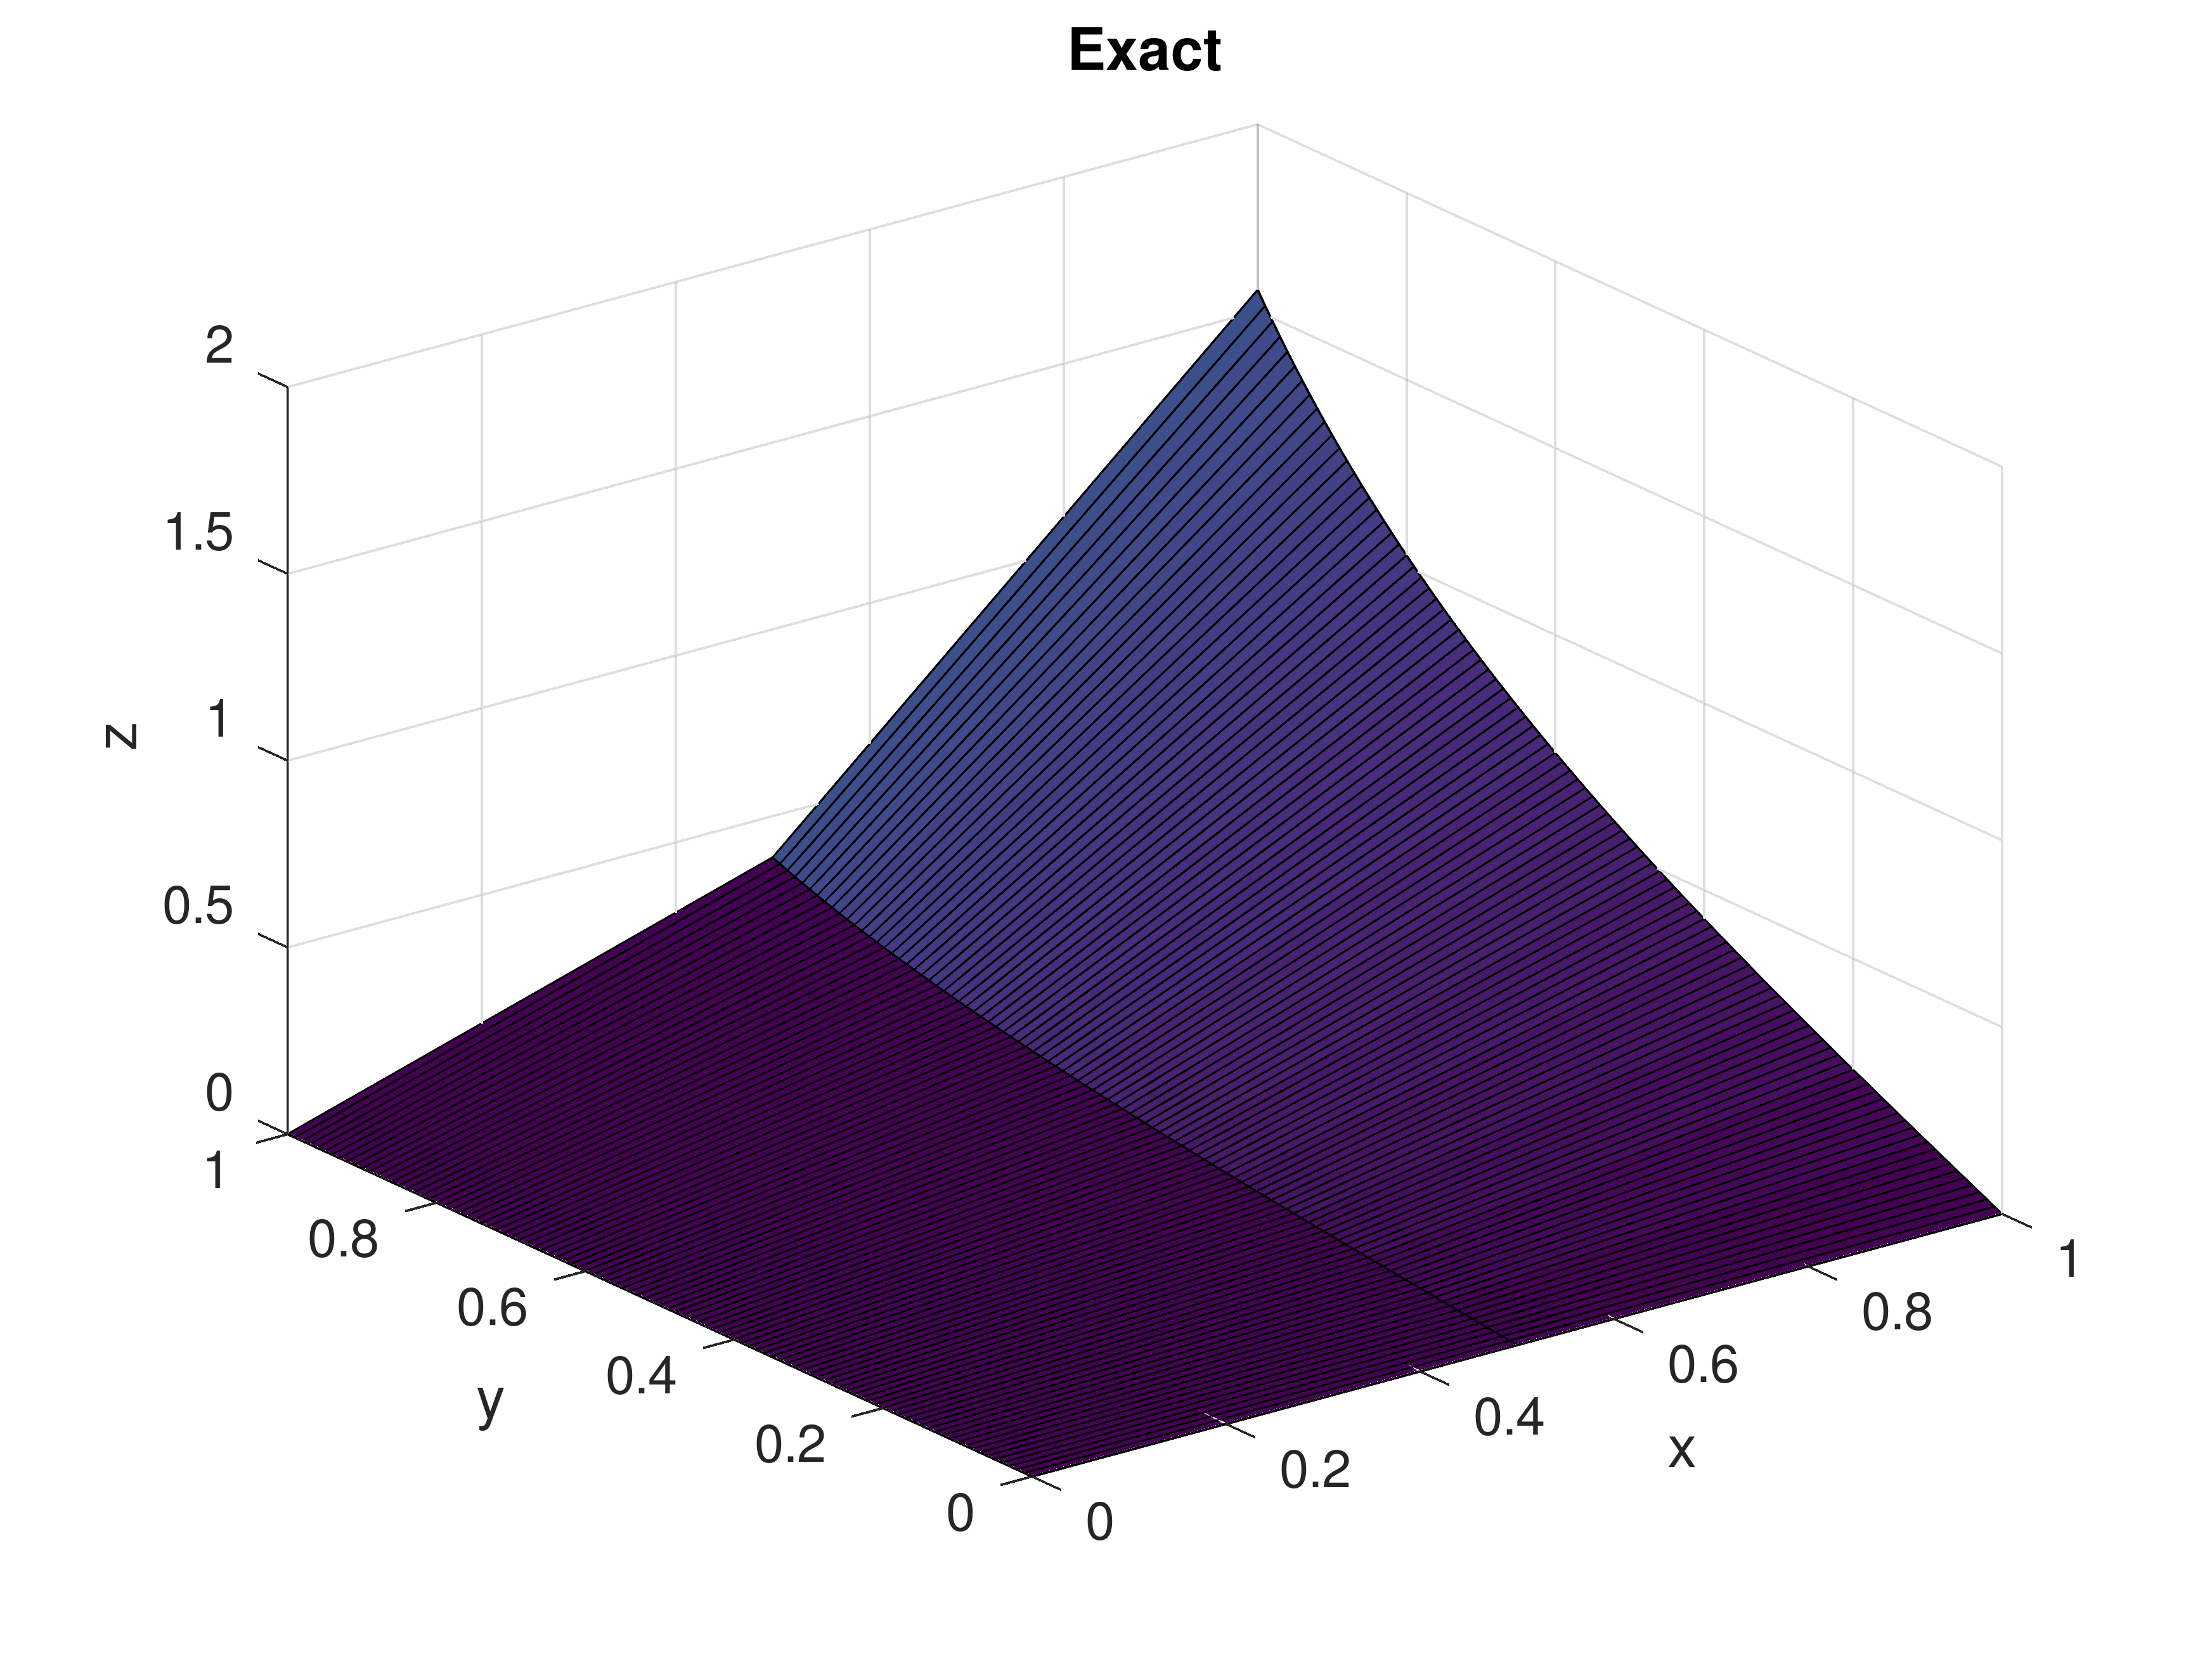
\includegraphics[scale=0.05]{Figures/firstExactN3}
			\caption{Exact}
		\end{subfigure}
		\qquad \begin{subfigure}{0.3\textwidth}
			%   \centering
			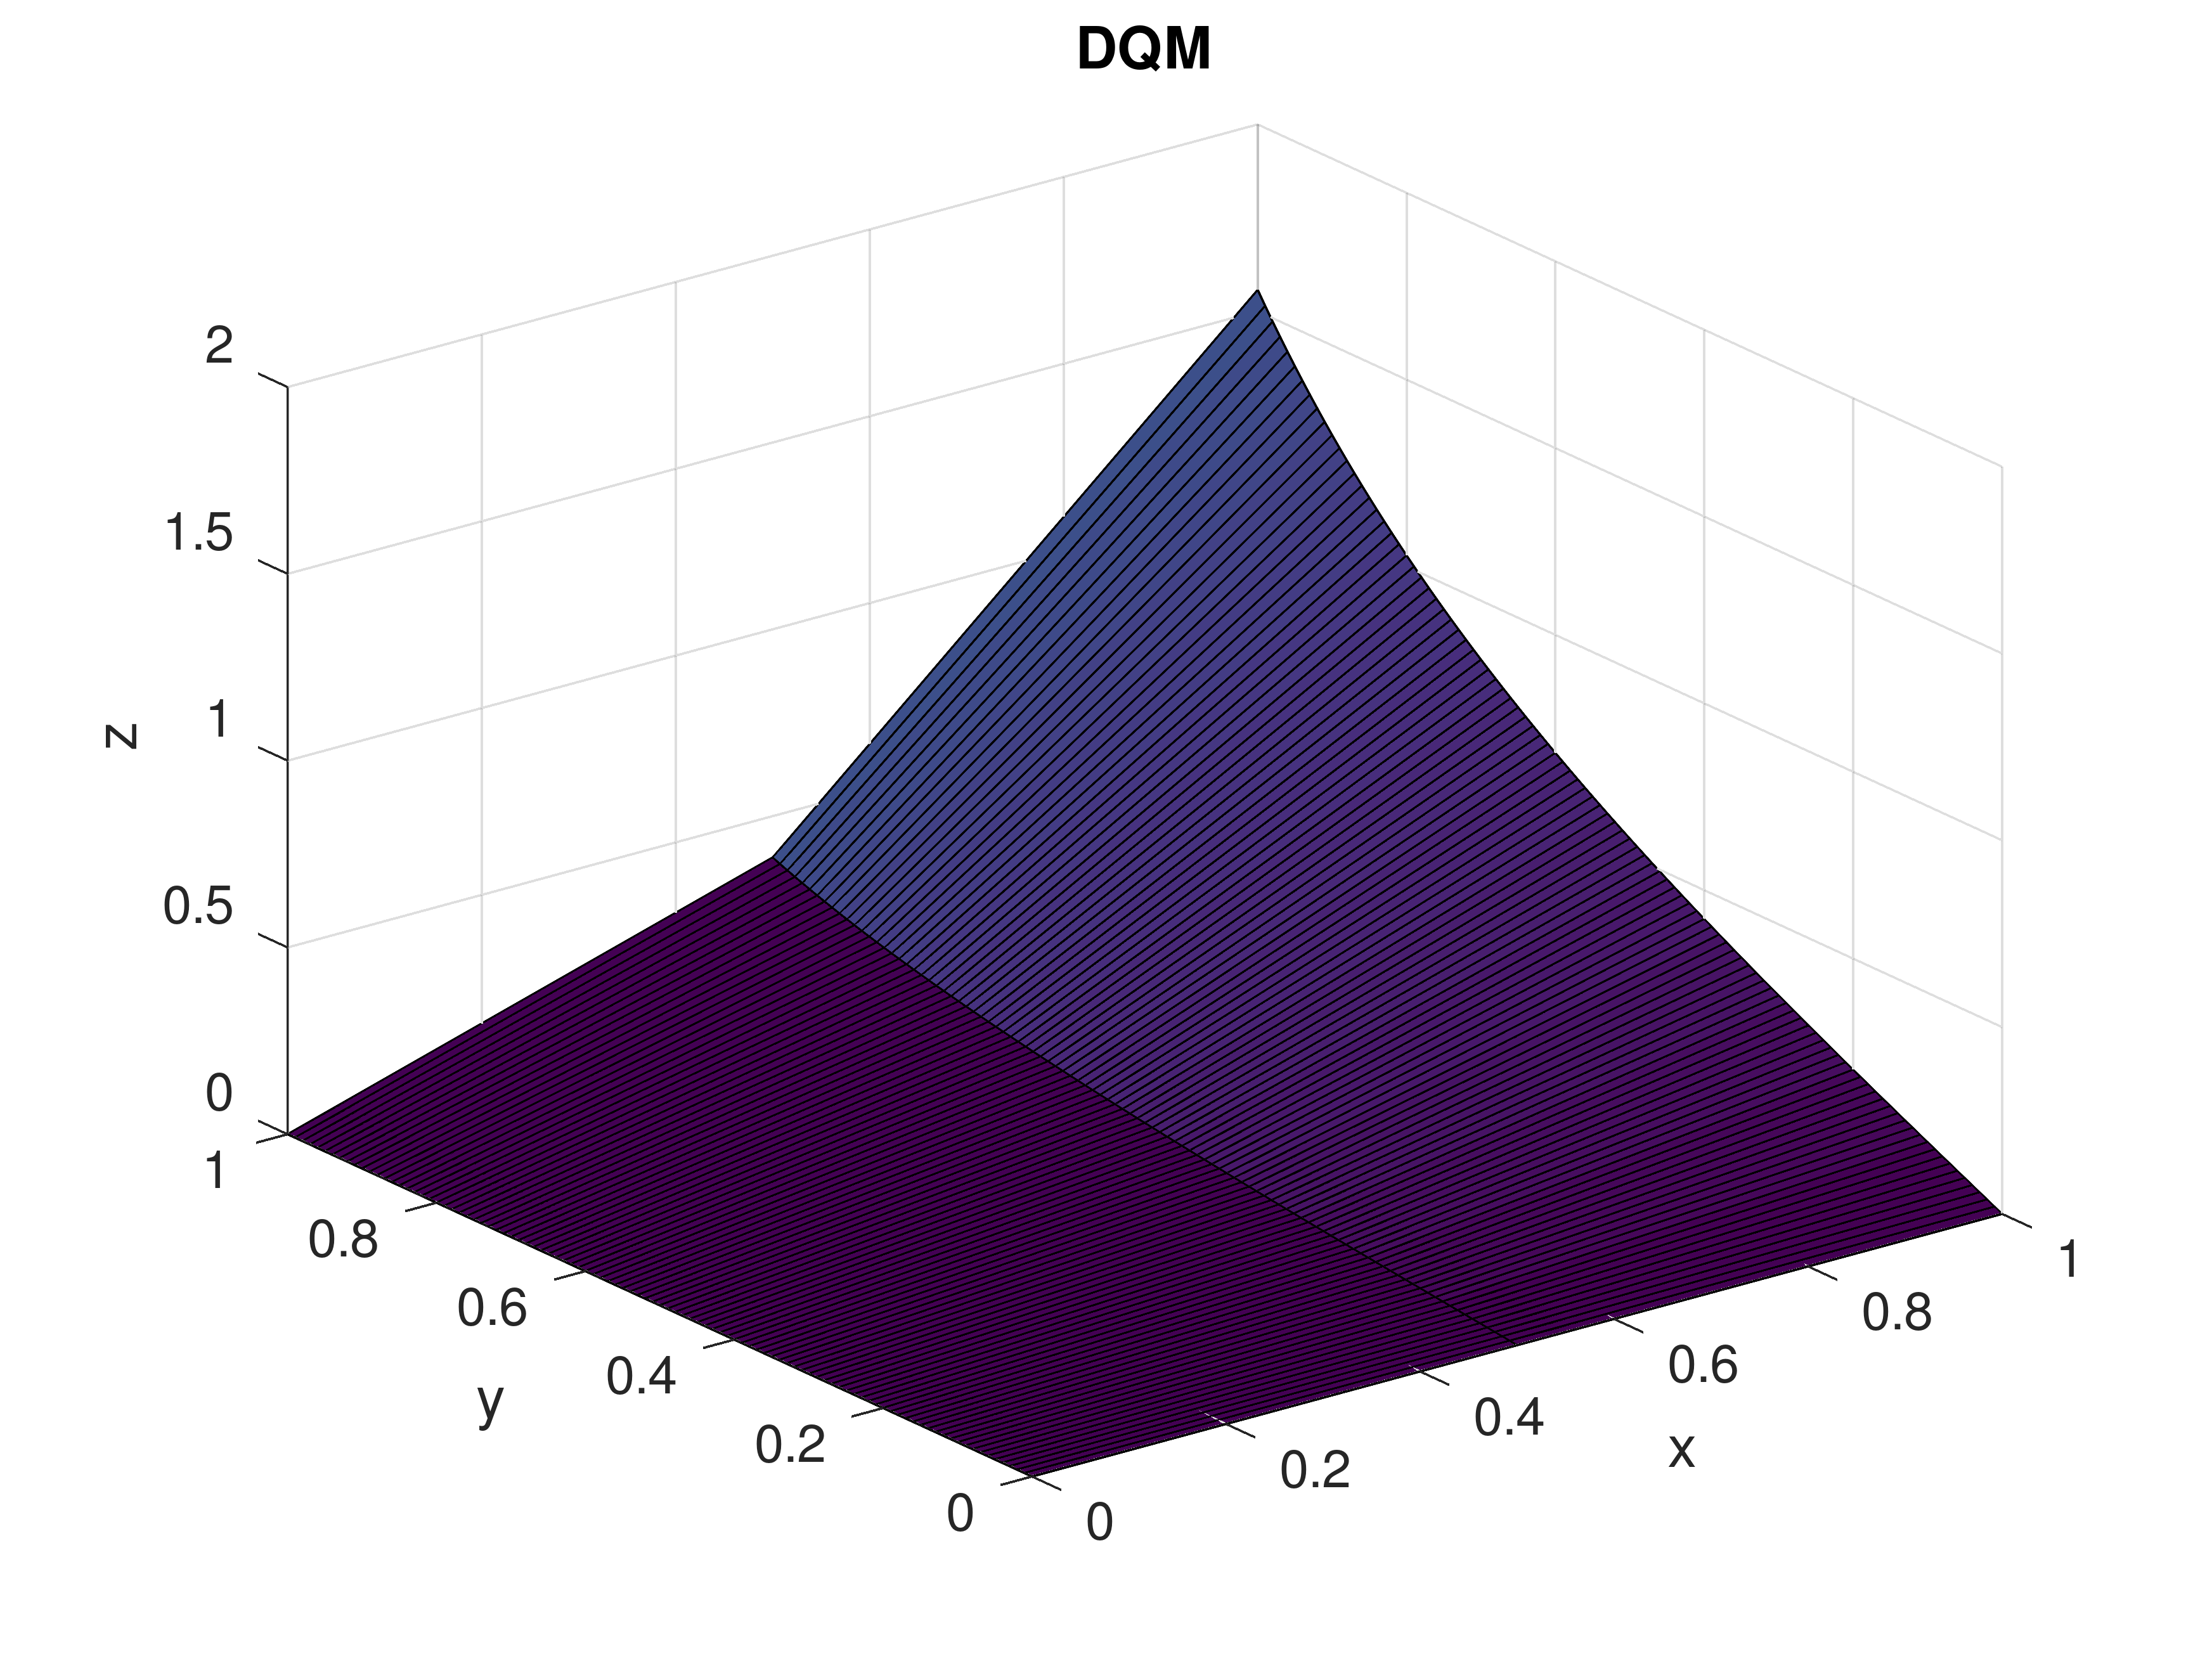
\includegraphics[scale=0.05]{Figures/firstN3}
			\caption{DQM}
		\end{subfigure}
		\caption{$N=3$ for the equation $u_t = x^2 + \frac{1}{4} u_t^2$}
		\label{fig:firstexampleN3}
	\end{figure}
\end{english}
الآن نأخذ $N=7$. نحسب معاملات الوزن من \eqref{quan_chang_equations}  
\[
\begin{bmatrix}
	-14.7 & 36 & -45 & 40 & -22.5 & 7.2 & -1 \\
	-1 & -7.7 & 15 & -10 & 5 & -1.5 & 0.2 \\
	0.2 & -2.4 & -3.5 & 8 & -3 & 0.8 & -0.1 \\
	-0.1 & 0.9 & -4.5 & -2.6645e-15 & 4.5 & -0.9 & 0.1 \\
	0.1 & -0.8 & 3 & -8 & 3.5 & 2.4 & -0.2 \\
	-0.2 & 1.5 & -5 & 10 & -15 & 7.7 & 1 \\
	1 & -7.2 & 22.5 & -40 & 45 & -36 & 14.7
\end{bmatrix}
\]
نعوض في \eqref{eq:firstexampleDQM} ونكمل الحل بواسطة \textbf{(RK4)} ينتج الحل في الجدول \ref{tab:firstexN7}.
\begin{english}
	\begin{table}[ht]
		\centering
		\begin{tabular}{|c|c|c|c|c|}
			\hline
			$t$ & $x_i$ & DQM & Exact & Error \\
			\hline
			\multirow{7}{*}{0.1} & $x_1$ & $4.7266 \times 10^{-34}$ & 0.0000 & $4.7266 \times 10^{-34}$ \\
			& $x_2$ & 0.0028 & 0.0028 & $2.3058 \times 10^{-9}$ \\
			& $x_3$ & 0.0111 & 0.0111 & $9.2230 \times 10^{-9}$ \\
			& $x_4$ & 0.0251 & 0.0251 & $2.0752 \times 10^{-8}$ \\
			& $x_5$ & 0.0446 & 0.0446 & $3.6892 \times 10^{-8}$ \\
			& $x_6$ & 0.0697 & 0.0697 & $5.7644 \times 10^{-8}$ \\
			& $x_7$ & 0.1003 & 0.1003 & $8.3007 \times 10^{-8}$ \\
			\hline
			\multirow{7}{*}{0.01} & $x_1$ & $9.2911 \times 10^{-37}$ & 0.0000 & $9.2911 \times 10^{-37}$ \\
			& $x_2$ & 0.0003 & 0.0003 & $2.3147 \times 10^{-14}$ \\
			& $x_3$ & 0.0011 & 0.0011 & $9.2589 \times 10^{-14}$ \\
			& $x_4$ & 0.0025 & 0.0025 & $2.0833 \times 10^{-13}$ \\
			& $x_5$ & 0.0044 & 0.0044 & $3.7036 \times 10^{-13}$ \\
			& $x_6$ & 0.0069 & 0.0069 & $5.7868 \times 10^{-13}$ \\
			& $x_7$ & 0.0100 & 0.0100 & $8.3330 \times 10^{-13}$ \\
			\hline
		\end{tabular}
		\caption{$N=7$}
		\label{tab:firstexN7}
	\end{table}
\end{english}

\begin{english}
	\begin{figure}[ht]
		\centering
		\begin{subfigure}{0.3\textwidth}
			%  \centering
			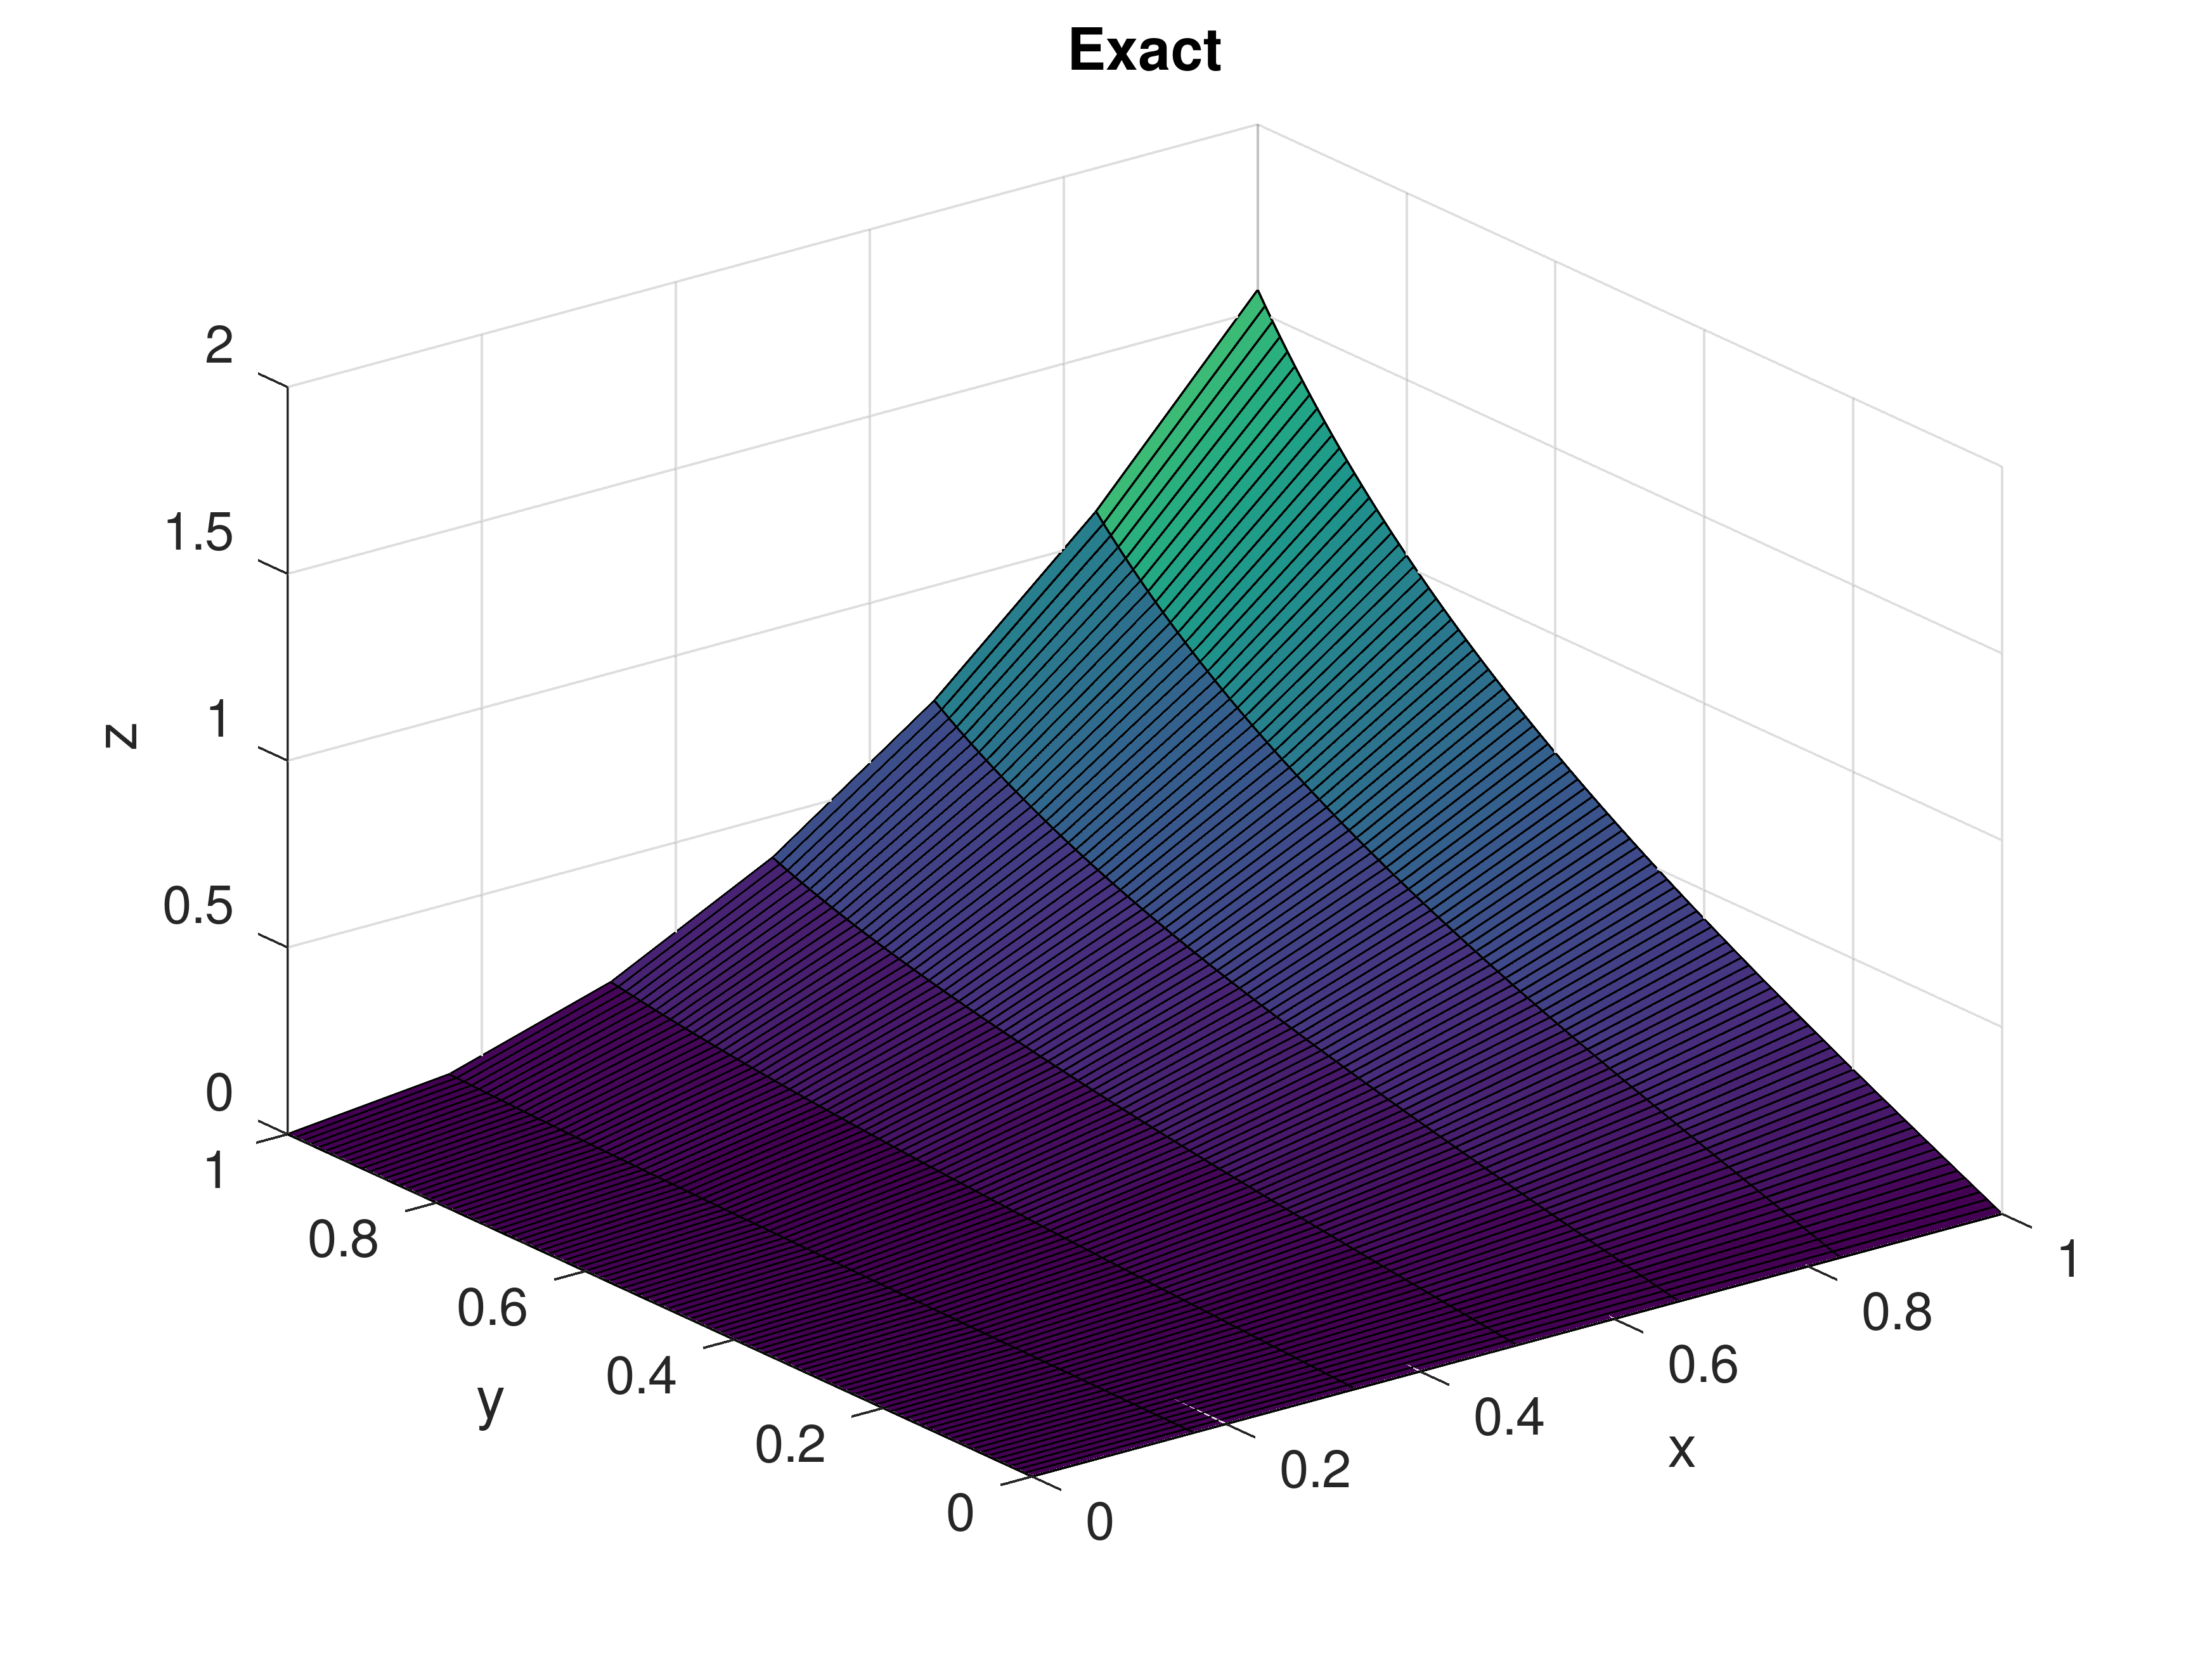
\includegraphics[scale=0.05]{Figures/firstExactN7}
			\caption{Exact}
		\end{subfigure}
		\qquad \begin{subfigure}{0.3\textwidth}
			%   \centering
			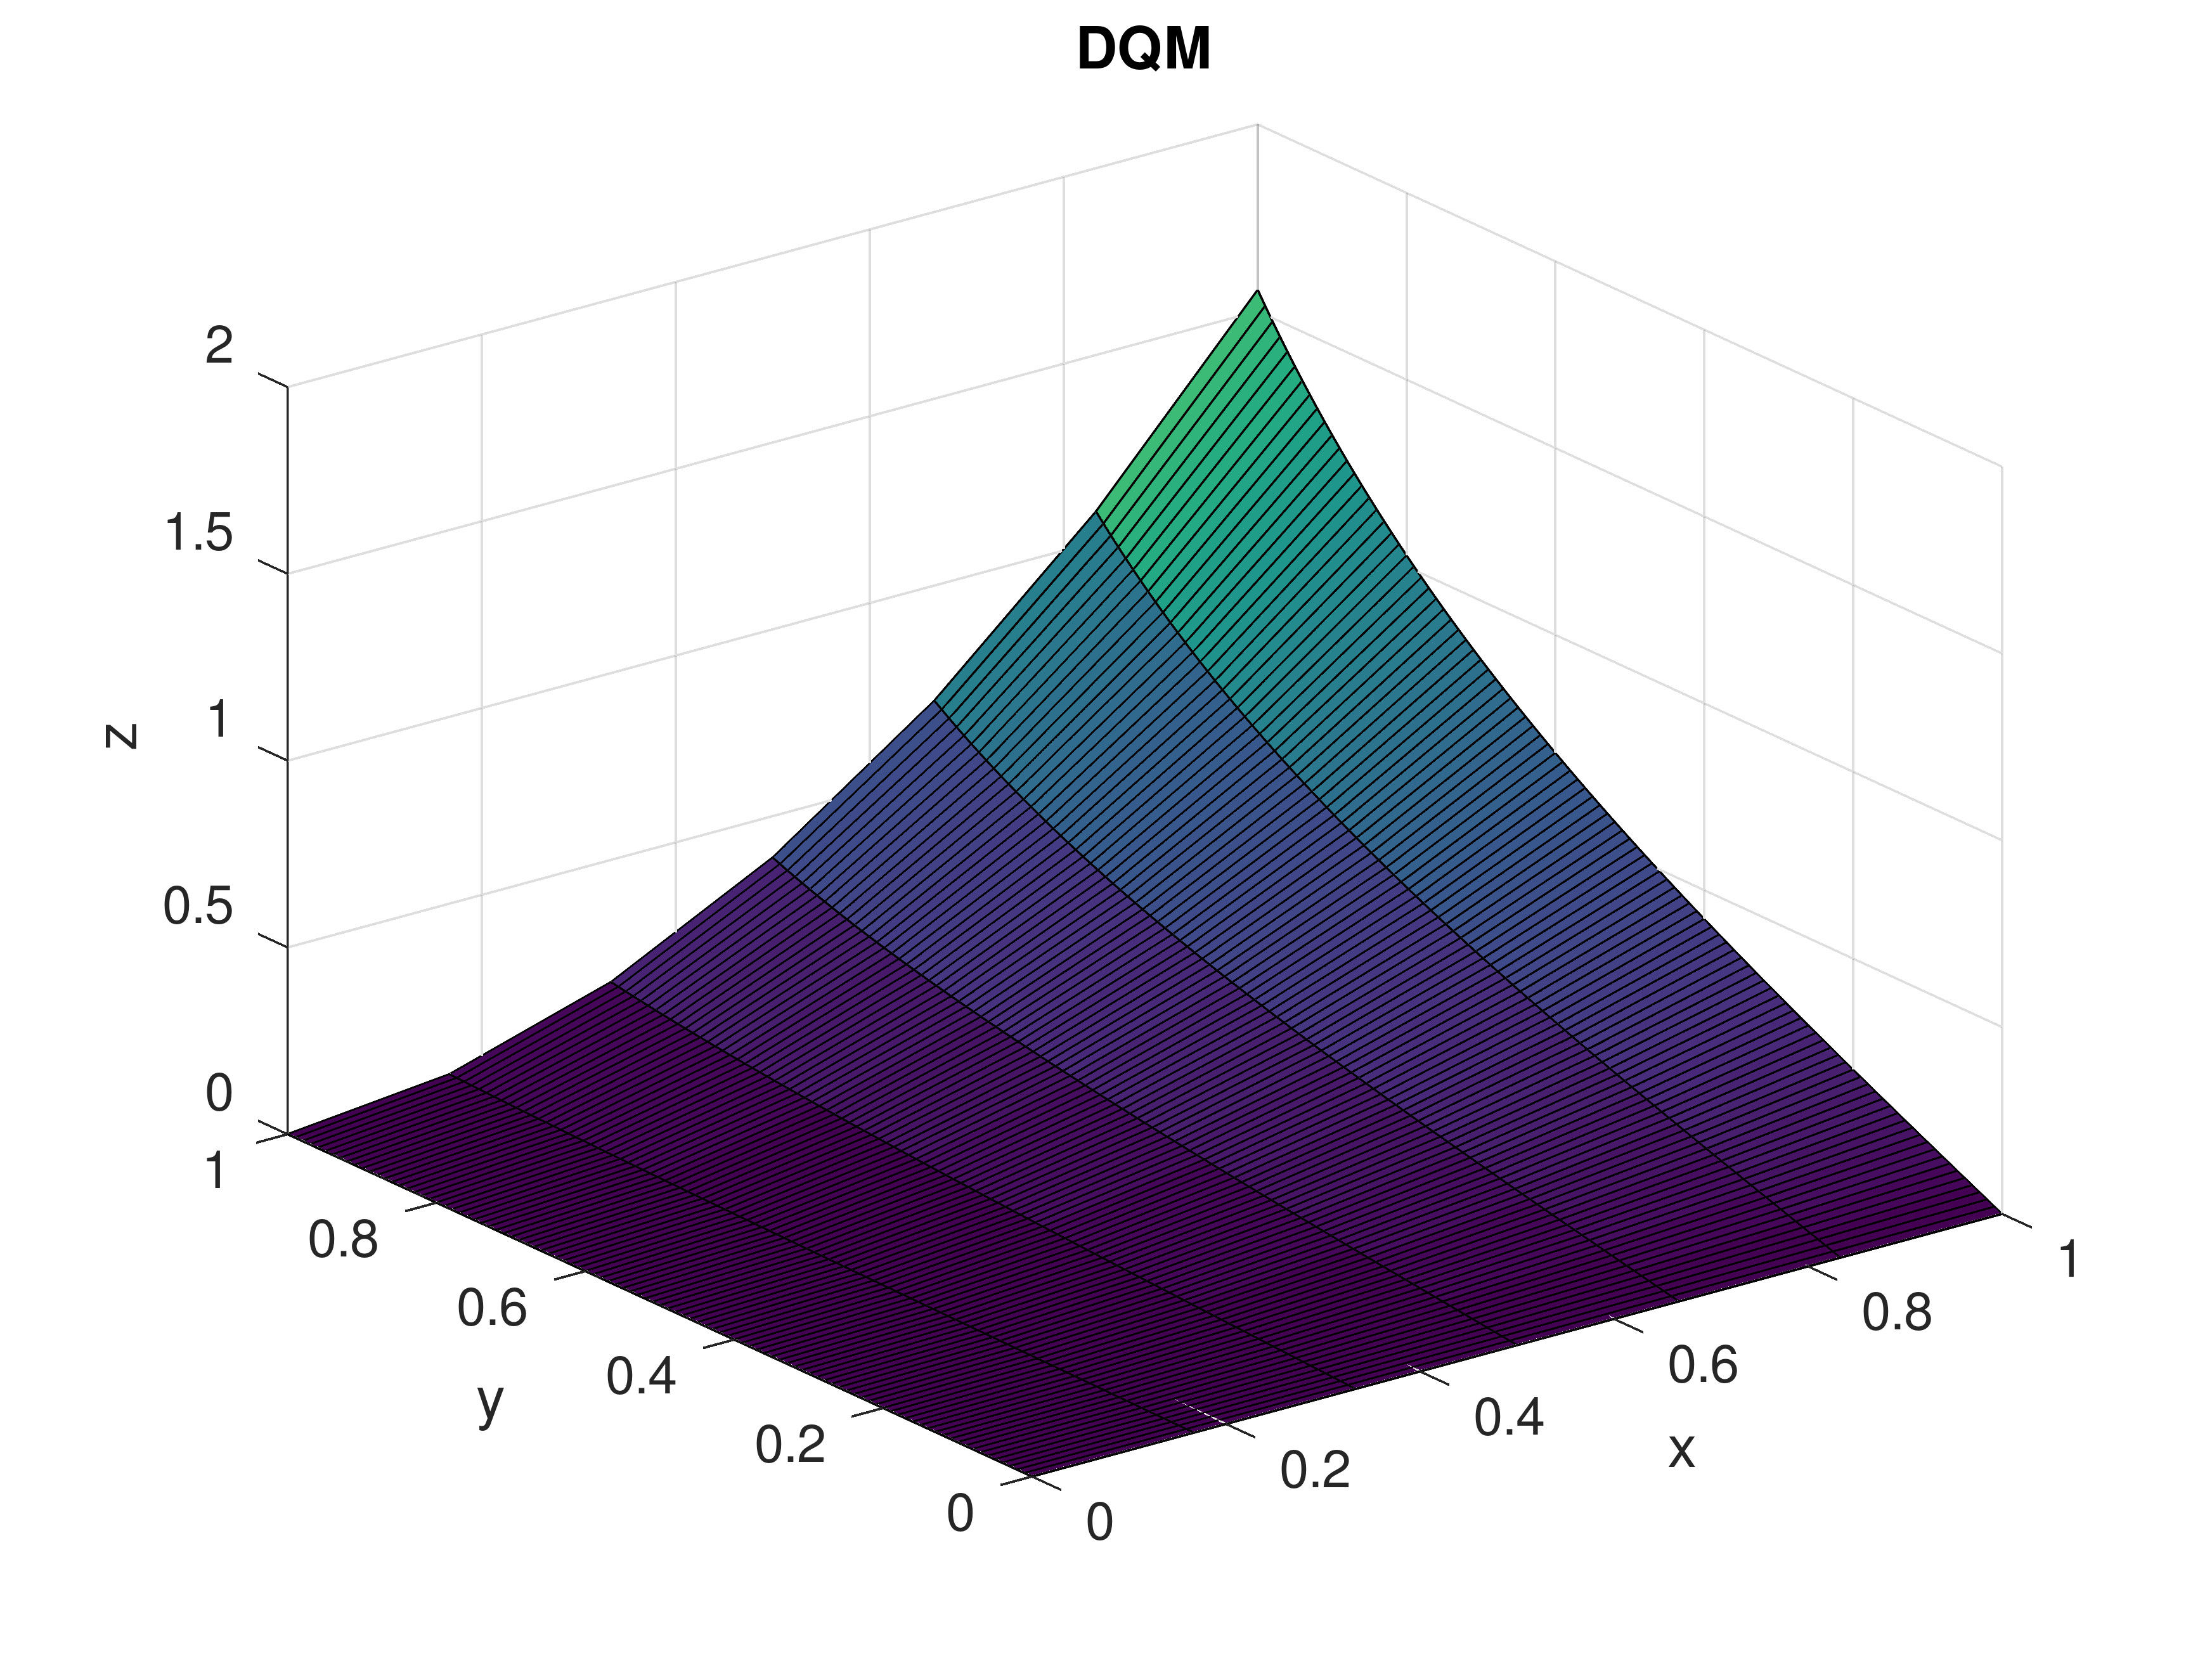
\includegraphics[scale=0.05]{Figures/firstN7}
			\caption{DQM}
		\end{subfigure}
		\caption{$N=7$ for the equation $u_t = x^2 + \frac{1}{4} u_t^2$}
		\label{fig:firstexampleN7}
	\end{figure}
\end{english}
\end{solution}


\begin{example}
	جد حل المعادلة باستخدام طريقة التفاضل التربيعي 
\begin{equation}
	\label{eq:secondexample}
		u_t + u u_x = x, \quad u(x, 0) = 2
\end{equation}
\end{example}
\begin{solution}
	نقوم باعادة  ترتيب المعادلة ونعوض التفاضل التربيعي للمشتقة بالنسبة الى $x$ في \eqref{eq:secondexample} نحصل على 
	\begin{equation}
		\label{eq:secondexampleDQM}
		u_t(x_i, t) = - u(x_i, t) \sum_{j=1}^{N} a_{ij} u(x_j, t) + x_i,\quad i =1\dots,N 
	\end{equation}
	لنأخذ $N=5$ وبواسطة \eqref{quan_chang_equations} نحسب معاملات الوزن 
\[
[a_{ij}] =
\begin{bmatrix}
	-8.3333 & 16 & -12 & 5.3333 & -1 \\
	-1 & -3.3333 & 6 & -2 & 0.33333 \\
	0.33333 & -2.6667 & 0 & 2.6667 & -0.33333 \\
	-0.33333 & 2 & -6 & 3.3333 & 1 \\
	1 & -5.3333 & 12 & -16 & 8.3333
\end{bmatrix}
\]
بطريقة مماثلة في المثال الاول. نعوض معاملات الوزن في \eqref{eq:secondexampleDQM} وينتج نظام من المعادلات التفاضلية غير الخطية نحلها بطريقة RK4 ينتج الحل في الجدول \ref{tab:secondexN5}.
\begin{english}
	\begin{table}[h!]
	\centering
	\begin{tabular}{|c|c|c|c|c|}
		\hline
		$t$ & $x_i$ & DQM & Exact & Error \\
		\hline
		\multirow{5}{*}{0.1} & $x_1$ & 1.9900 & 1.9900 & $1.8168 \times 10^{-8}$ \\
		& $x_2$ & 2.0150 & 2.0150 & $3.9086 \times 10^{-8}$ \\
		& $x_3$ & 2.0399 & 2.0399 & $6.0004 \times 10^{-8}$ \\
		& $x_4$ & 2.0648 & 2.0648 & $8.0922 \times 10^{-8}$ \\
		& $x_5$ & 2.0897 & 2.0897 & $1.0184 \times 10^{-7}$ \\
		\hline
		\multirow{5}{*}{0.01} & $x_1$ & 1.9999 & 1.9999 & $1.7986 \times 10^{-14}$ \\
		& $x_2$ & 2.0024 & 2.0024 & $2.2604 \times 10^{-13}$ \\
		& $x_3$ & 2.0049 & 2.0049 & $4.3476 \times 10^{-13}$ \\
		& $x_4$ & 2.0074 & 2.0074 & $6.4304 \times 10^{-13}$ \\
		& $x_5$ & 2.0099 & 2.0099 & $8.5132 \times 10^{-13}$ \\
		\hline
	\end{tabular}
	\caption{$N=5$}
	\label{tab:secondexN5}
\end{table}
\end{english}
\begin{english}
	\begin{figure}[ht]
		\centering
		\begin{subfigure}{0.3\textwidth}
			%  \centering
			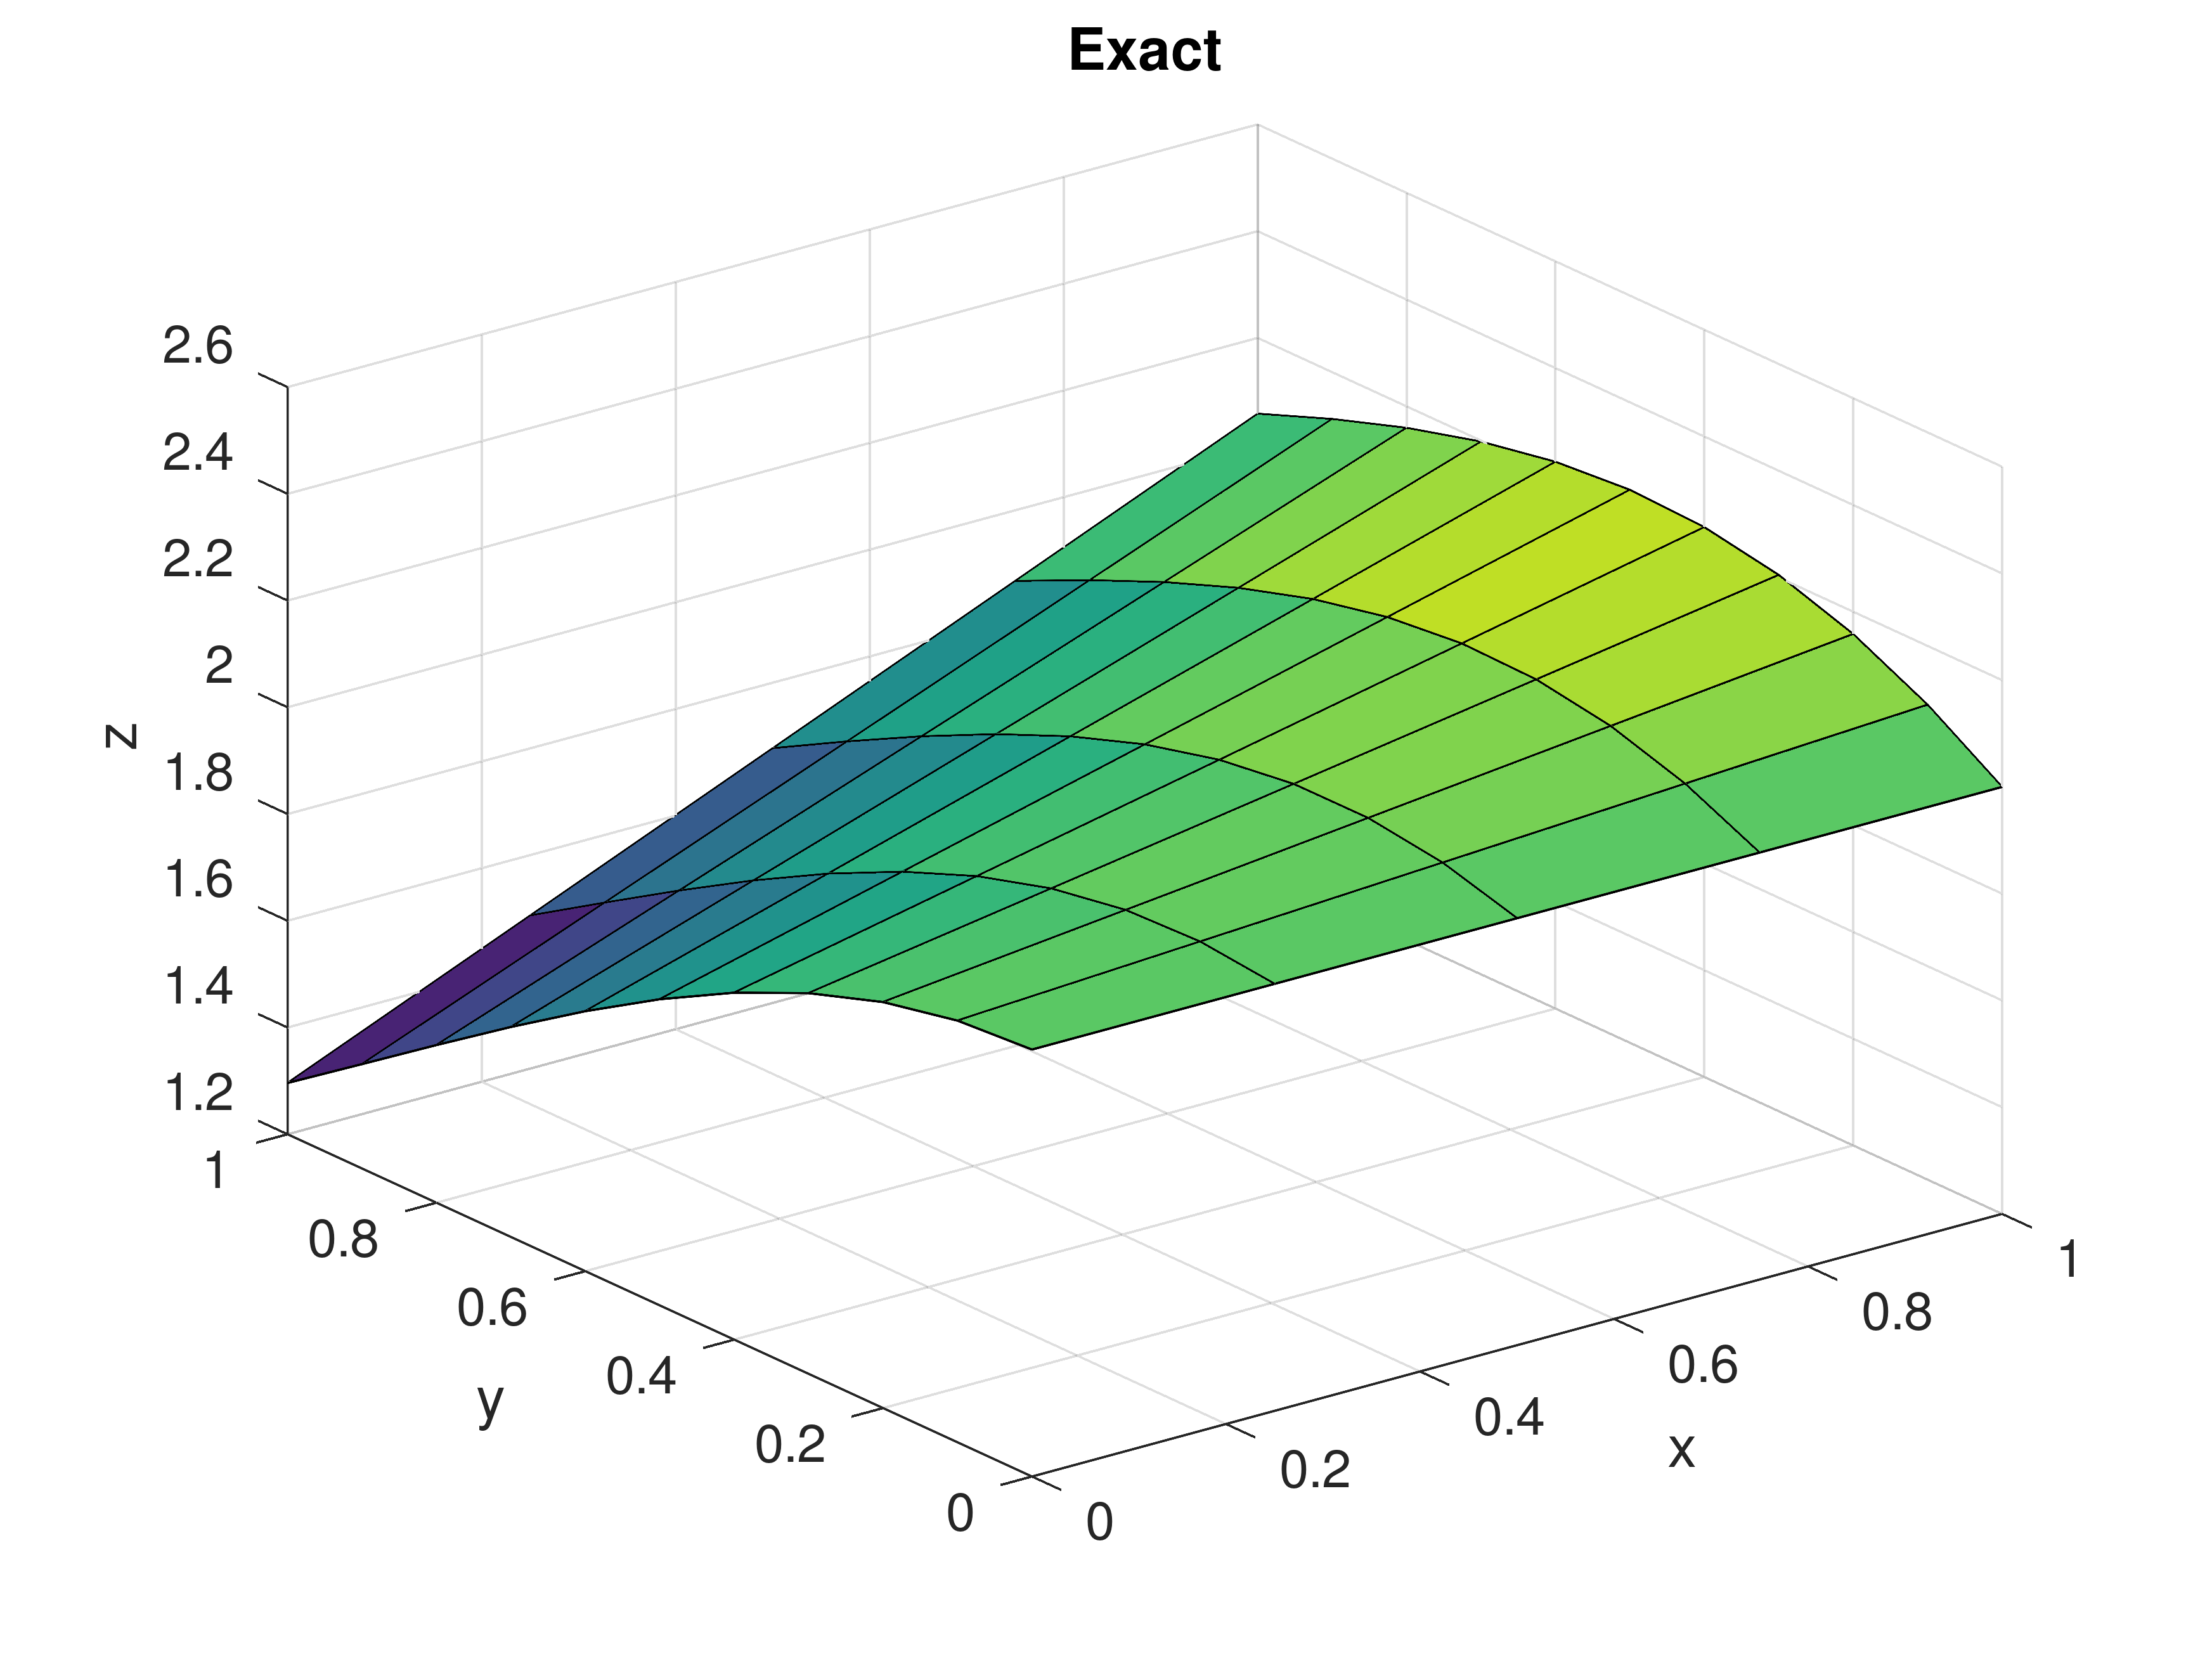
\includegraphics[scale=0.05]{Figures/secondExactN5}
			\caption{Exact}
		\end{subfigure}
		\qquad \begin{subfigure}{0.3\textwidth}
			%   \centering
			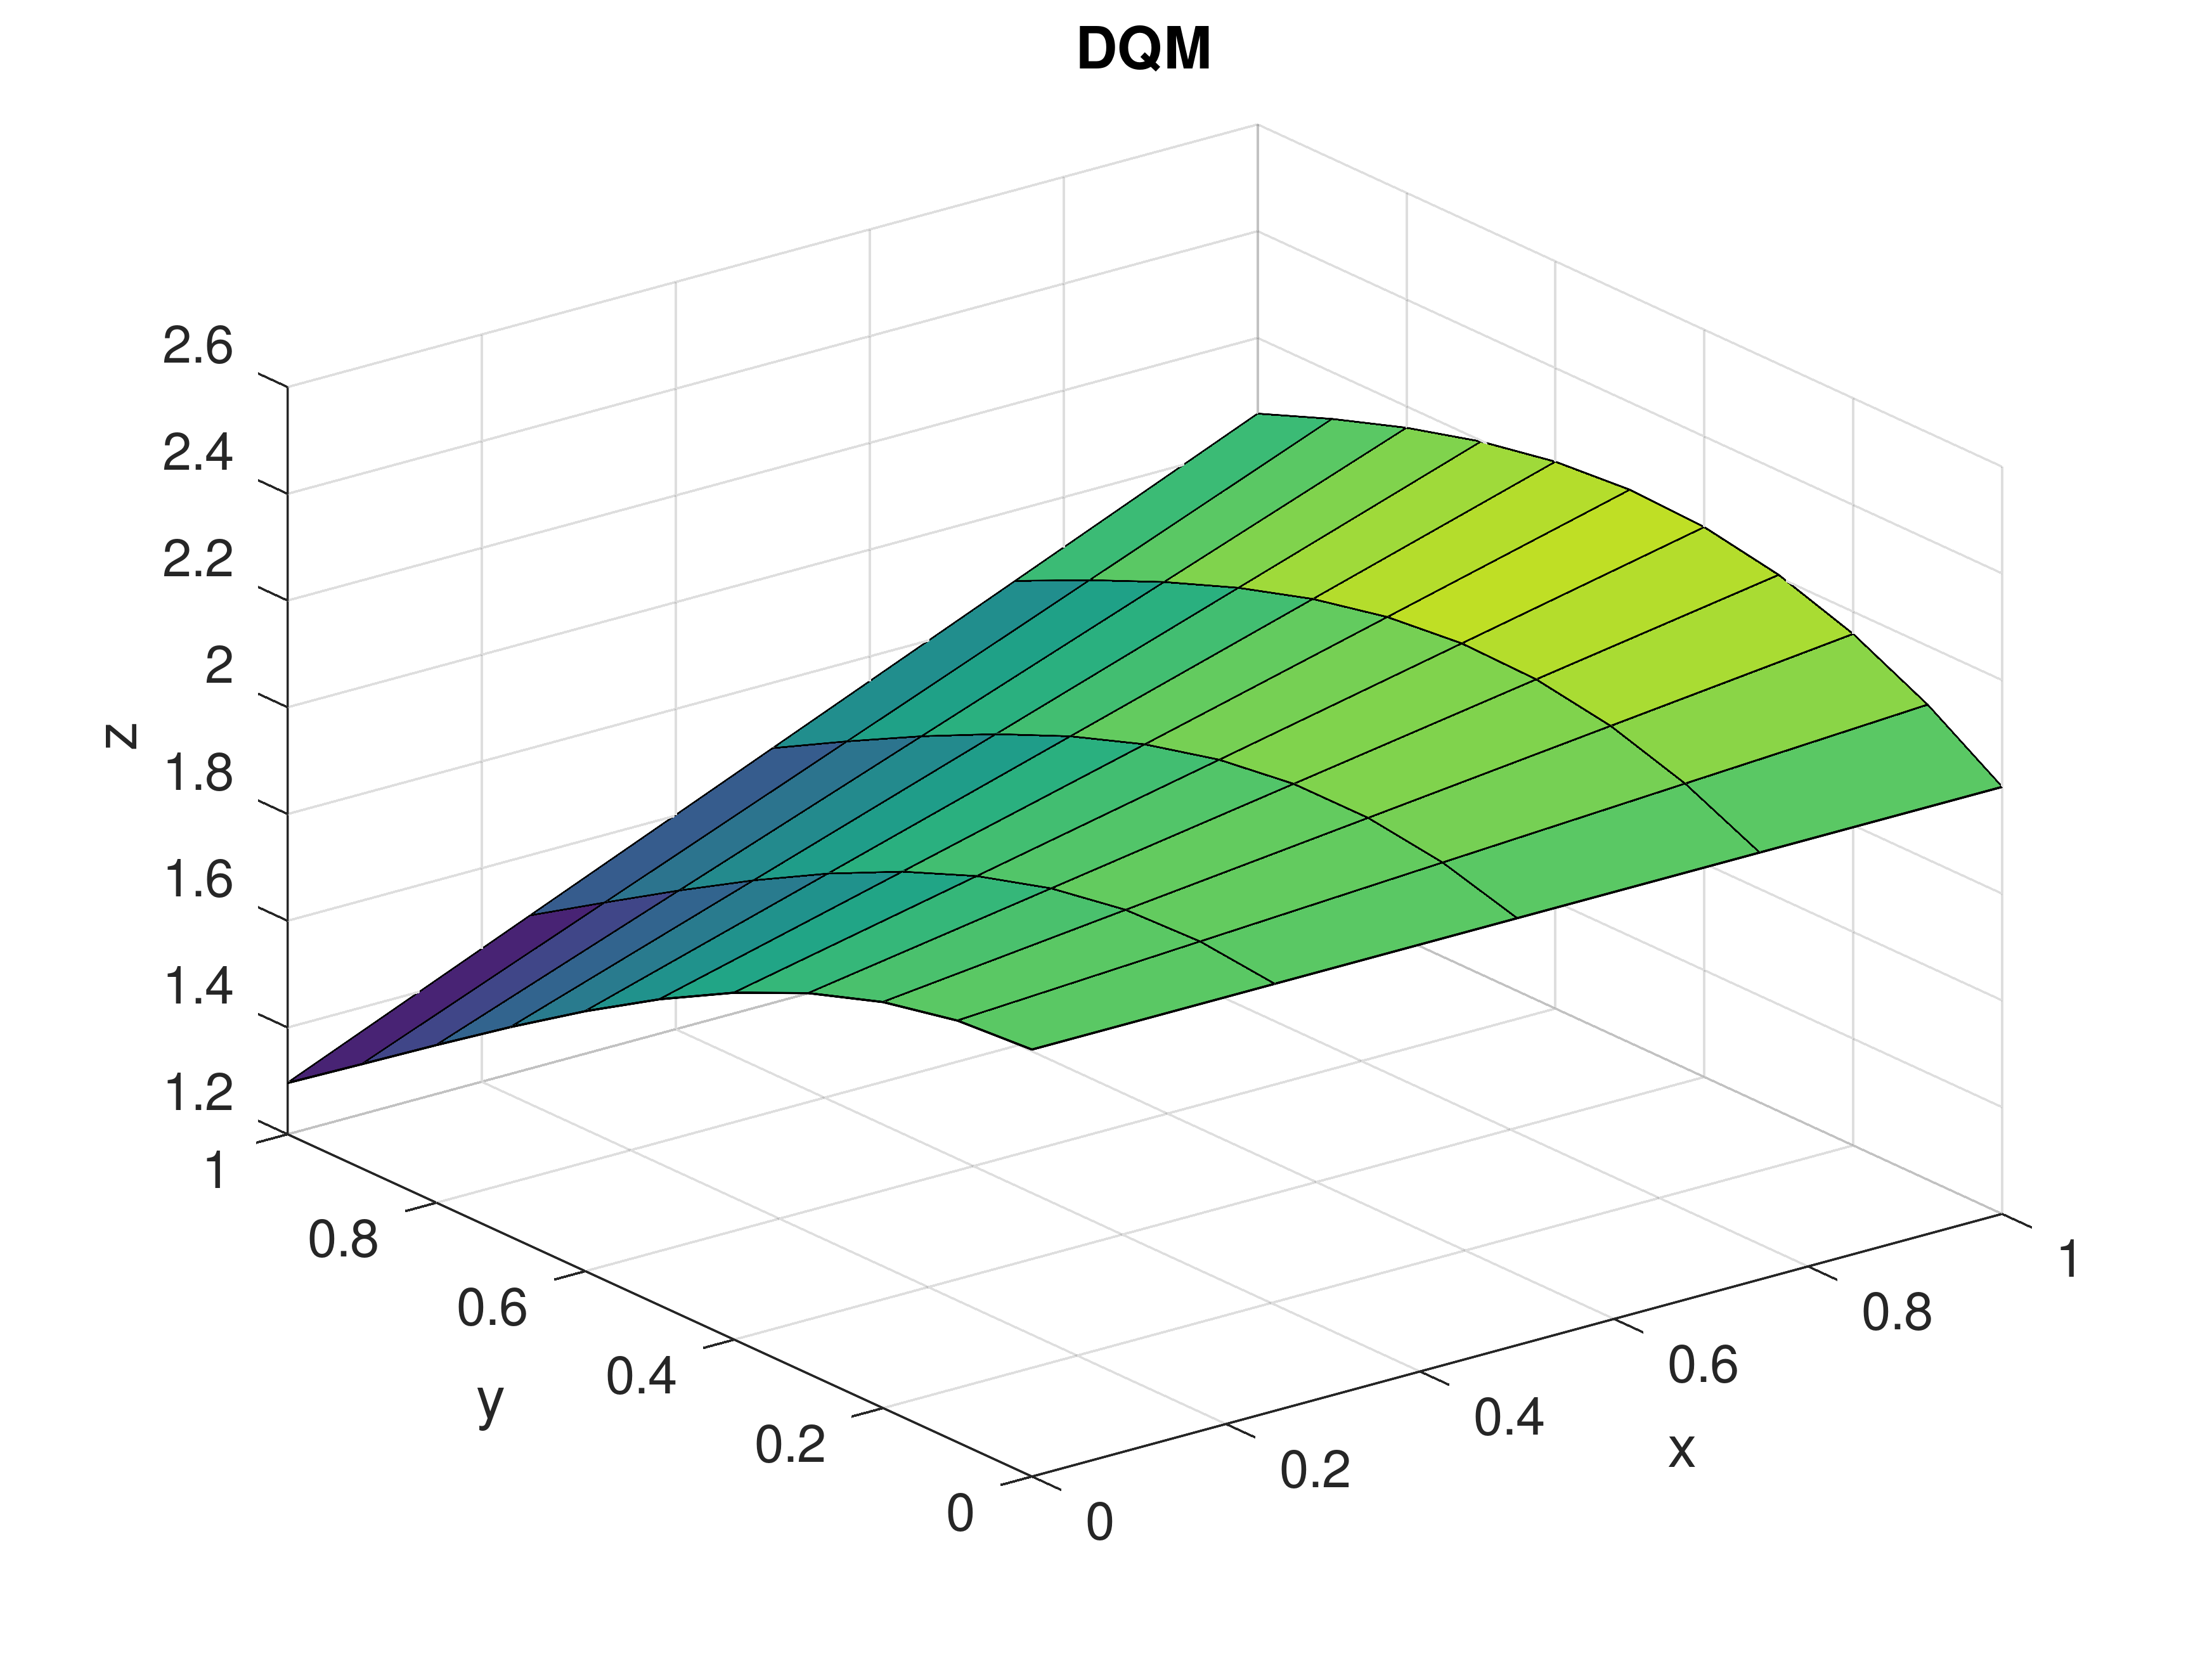
\includegraphics[scale=0.05]{Figures/secondN5}
			\caption{DQM}
		\end{subfigure}
		\caption{$N=5$ for the equation $u_t + u u_x = x$}
		\label{fig:secondexampleN5}
	\end{figure}
\end{english}
الآن لهدف المقارنة نأخذ $N=7$ ونحسب معاملات الوزن
\[
\begin{bmatrix}
	-14.7 & 36 & -45 & 40 & -22.5 & 7.2 & -1 \\
	-1 & -7.7 & 15 & -10 & 5 & -1.5 & 0.2 \\
	0.2 & -2.4 & -3.5 & 8 & -3 & 0.8 & -0.1 \\
	-0.1 & 0.9 & -4.5 & -2.6645e-15 & 4.5 & -0.9 & 0.1 \\
	0.1 & -0.8 & 3 & -8 & 3.5 & 2.4 & -0.2 \\
	-0.2 & 1.5 & -5 & 10 & -15 & 7.7 & 1 \\
	1 & -7.2 & 22.5 & -40 & 45 & -36 & 14.7
\end{bmatrix}
\]
ونحصل على الحل في الجدول \ref{tab:secondexN7}
\begin{english}
	\begin{table}[h!]
		\centering
		\begin{tabular}{|c|c|c|c|c|}
			\hline
			$t$ & $x_i$ & DQM & Exact & Error \\
			\hline
			\multirow{7}{*}{0.1} & $x_1$ & 1.9900 & 1.9900 & $1.8168 \times 10^{-8}$ \\
			& $x_2$ & 2.0067 & 2.0067 & $3.2114 \times 10^{-8}$ \\
			& $x_3$ & 2.0233 & 2.0233 & $4.6059 \times 10^{-8}$ \\
			& $x_4$ & 2.0399 & 2.0399 & $6.0004 \times 10^{-8}$ \\
			& $x_5$ & 2.0565 & 2.0565 & $7.3950 \times 10^{-8}$ \\
			& $x_6$ & 2.0731 & 2.0731 & $8.7895 \times 10^{-8}$ \\
			& $x_7$ & 2.0897 & 2.0897 & $1.0184 \times 10^{-7}$ \\
			\hline
			\multirow{7}{*}{0.01} & $x_1$ & 1.9999 & 1.9999 & $1.7097 \times 10^{-14}$ \\
			& $x_2$ & 2.0016 & 2.0016 & $1.5721 \times 10^{-13}$ \\
			& $x_3$ & 2.0032 & 2.0032 & $2.9576 \times 10^{-13}$ \\
			& $x_4$ & 2.0049 & 2.0049 & $4.3476 \times 10^{-13}$ \\
			& $x_5$ & 2.0066 & 2.0066 & $5.7332 \times 10^{-13}$ \\
			& $x_6$ & 2.0082 & 2.0082 & $7.1232 \times 10^{-13}$ \\
			& $x_7$ & 2.0099 & 2.0099 & $8.5043 \times 10^{-13}$ \\
			\hline
		\end{tabular}
		\caption{$N=7$}
	\label{tab:secondexN7}
	\end{table}
\end{english}

\begin{english}
	\begin{figure}[ht]
		\centering
		\begin{subfigure}{0.3\textwidth}
			%  \centering
			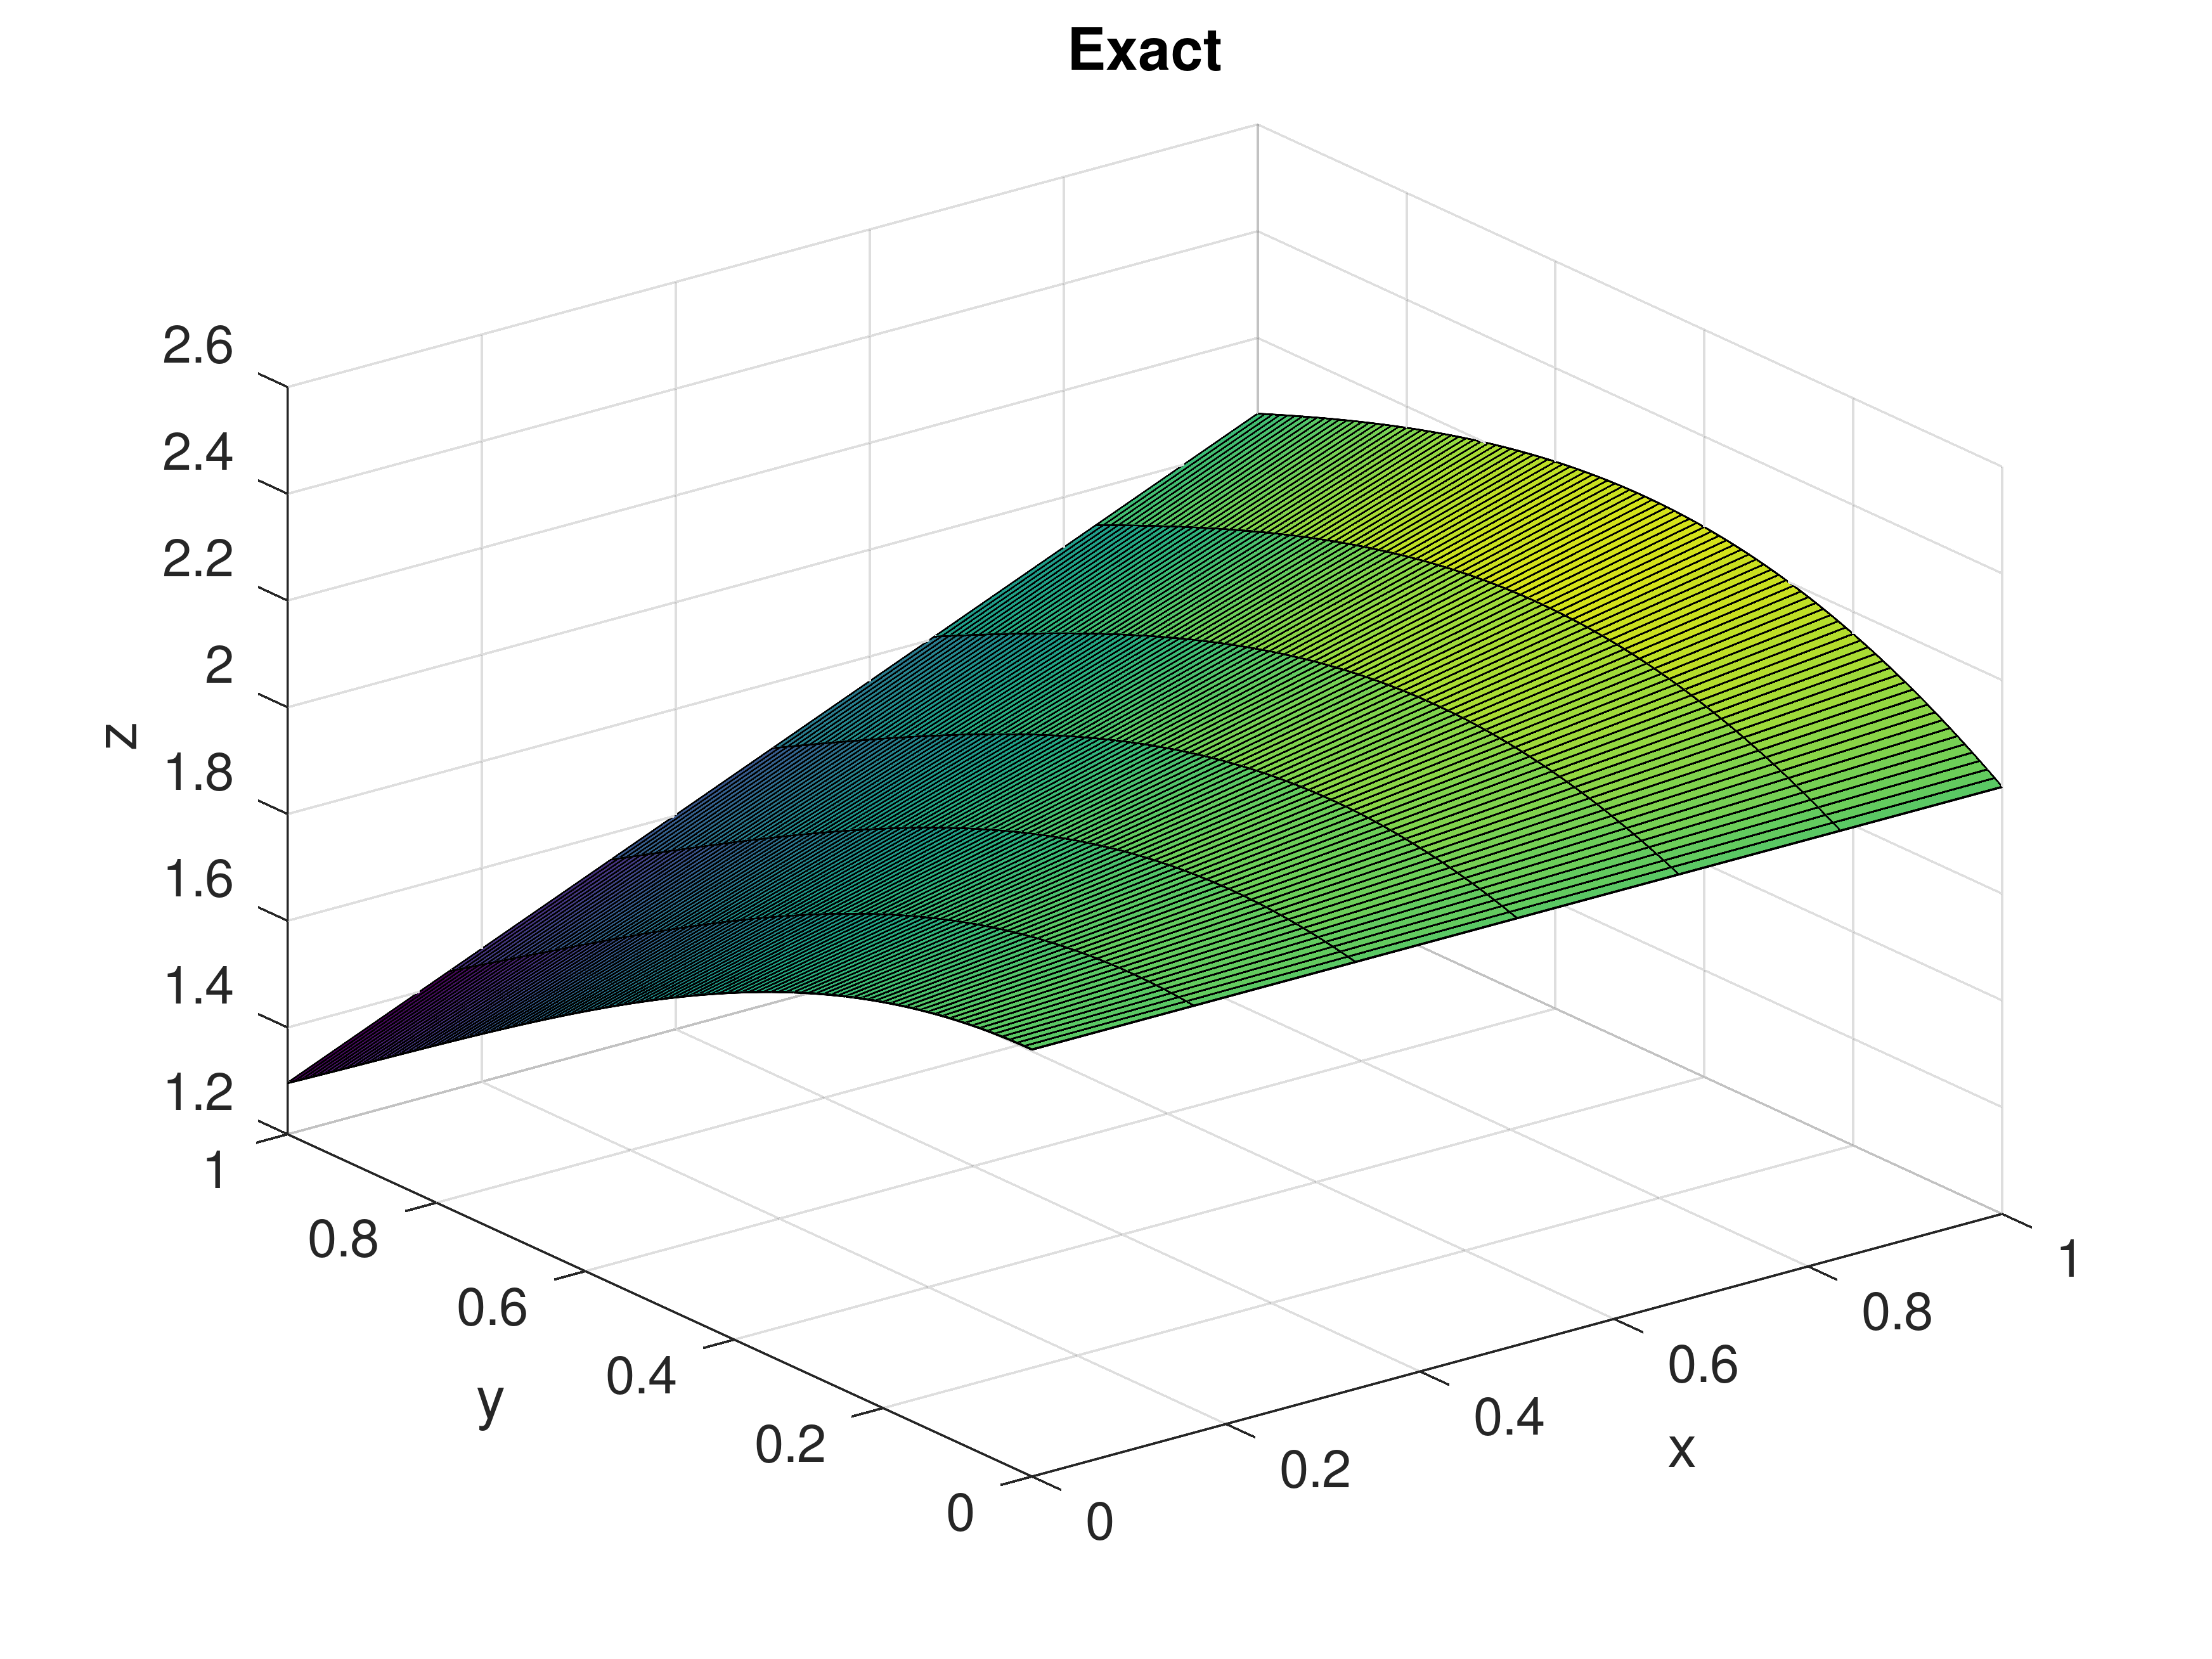
\includegraphics[scale=0.05]{Figures/secondExactN7}
			\caption{Exact}
		\end{subfigure}
		\qquad \begin{subfigure}{0.3\textwidth}
			%   \centering
			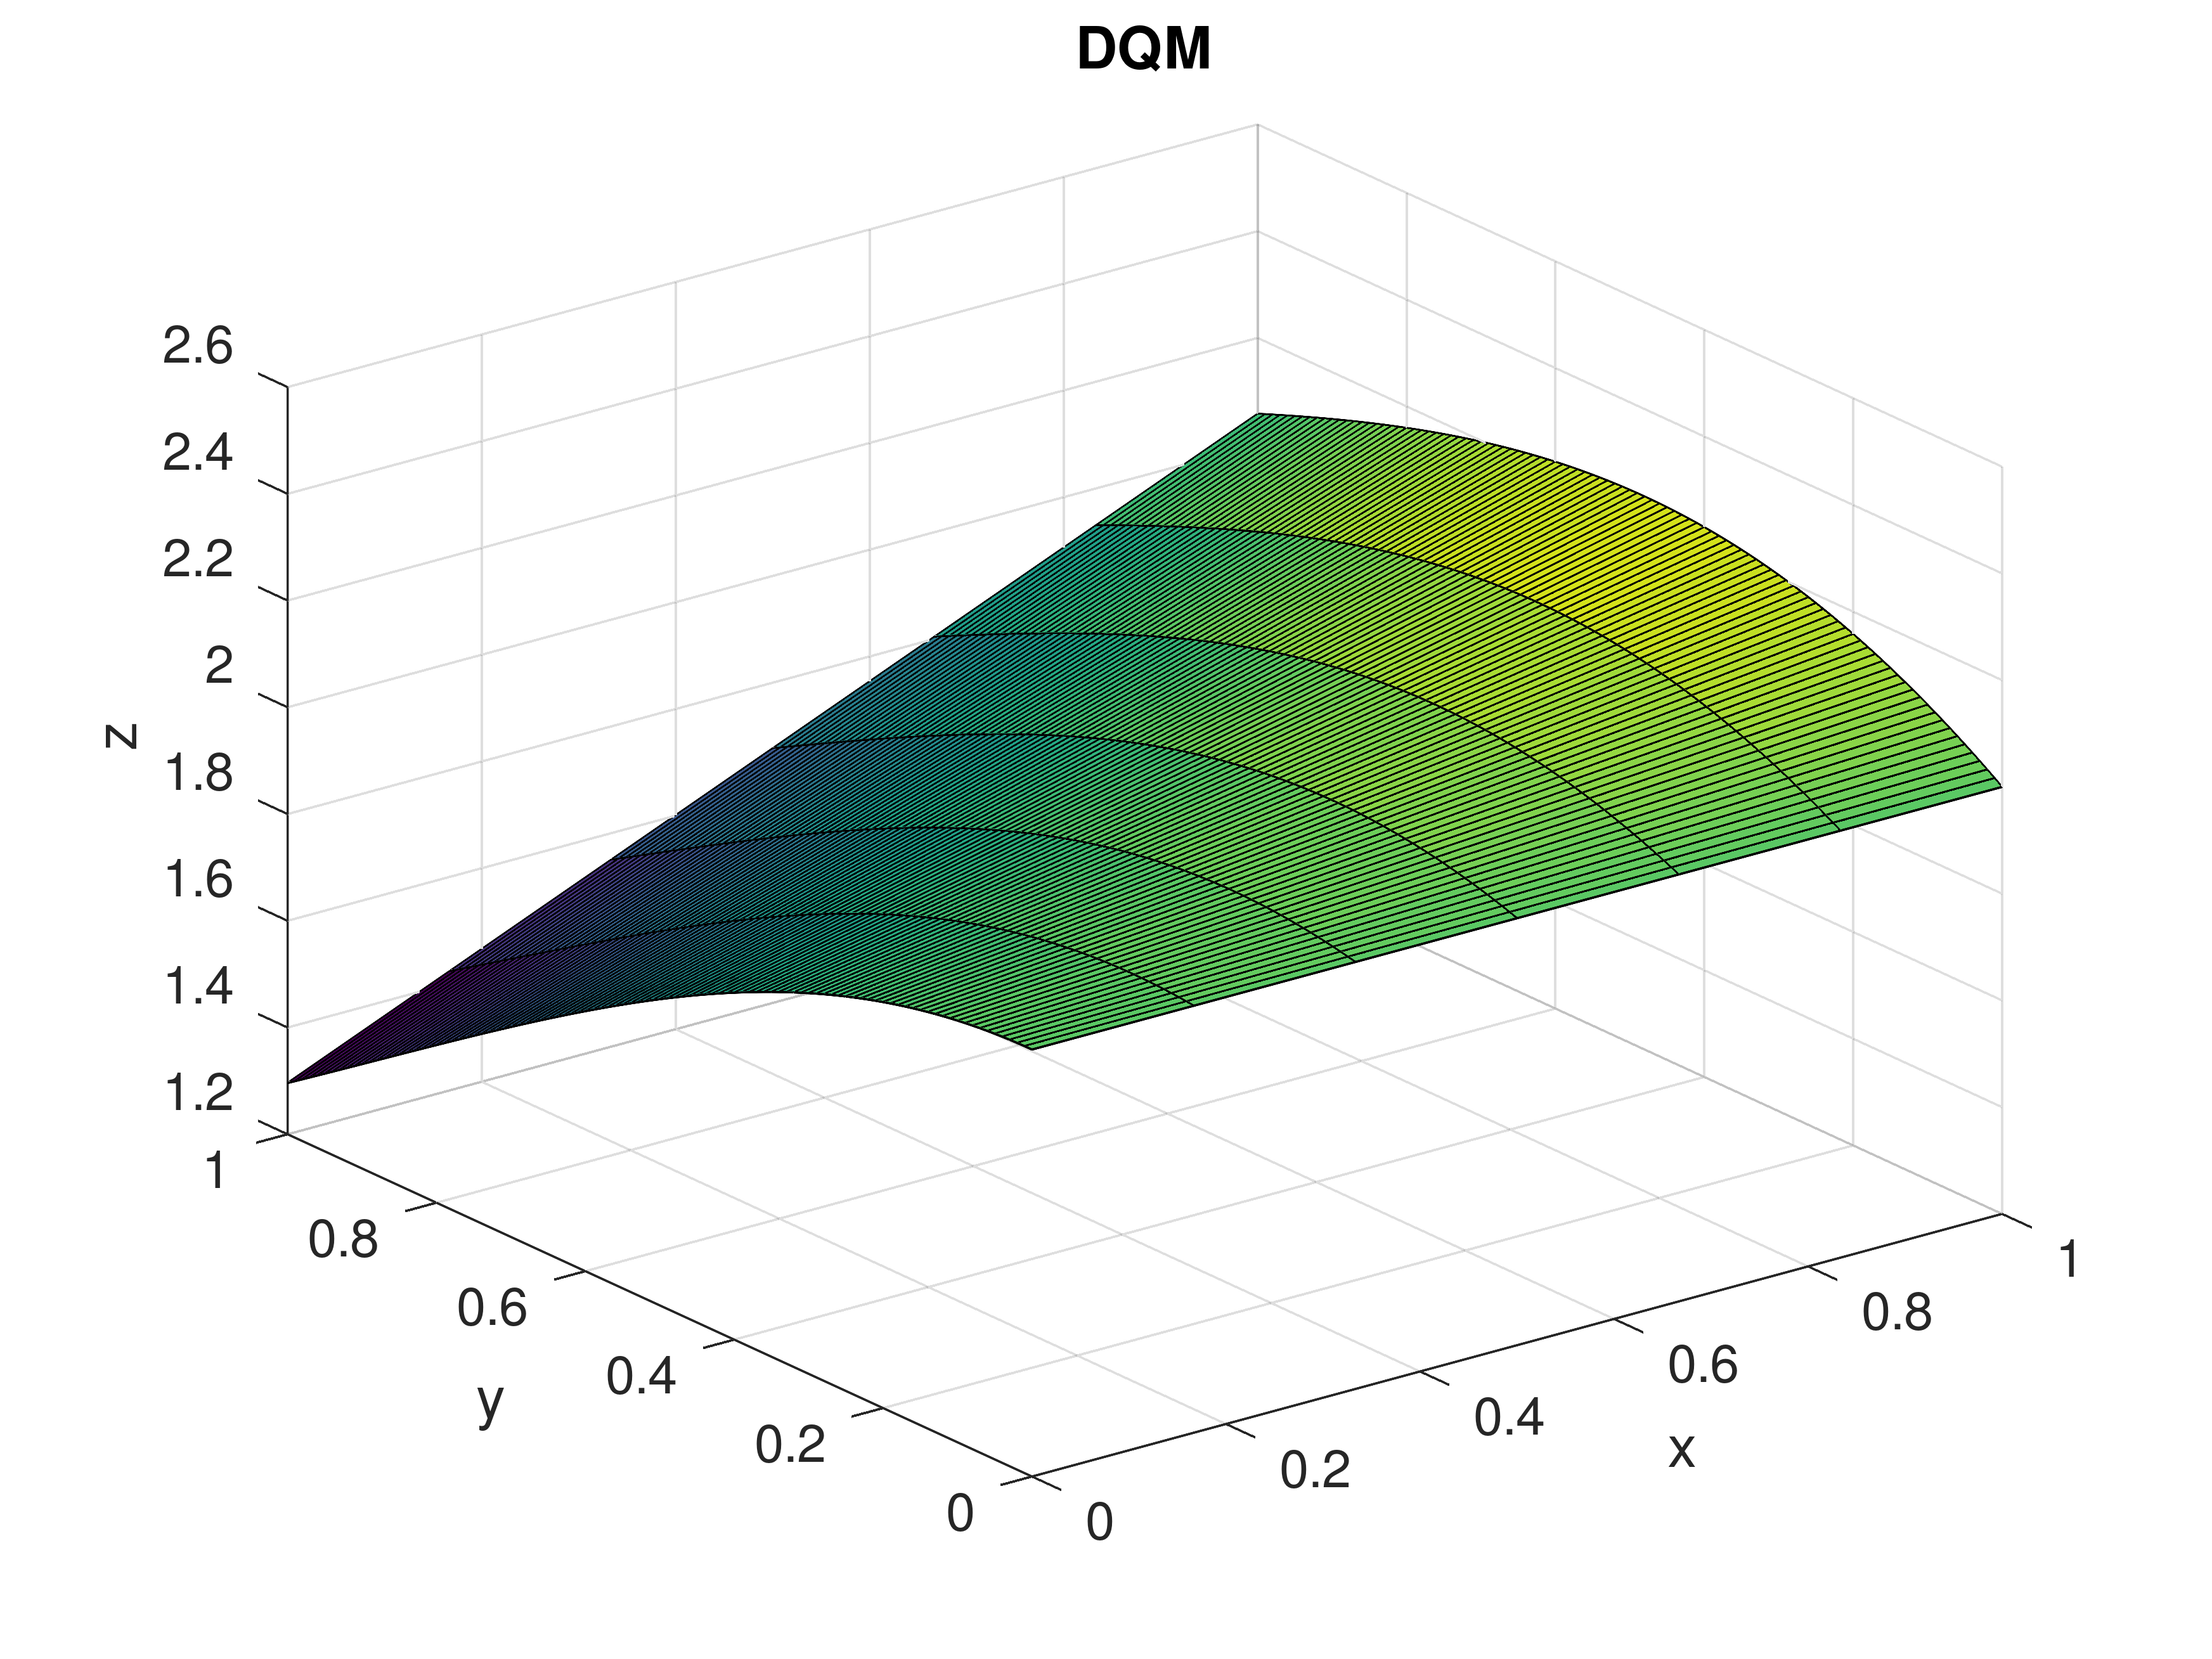
\includegraphics[scale=0.05]{Figures/secondN7}
			\caption{DQM}
		\end{subfigure}
		\caption{$N=7$ for the equation $u_t + u u_x = x$}
		\label{fig:secondexampleN7}
	\end{figure}
\end{english}
\end{solution}